\documentclass[10pt,usenames,dvipsnames]{article}

\usepackage{amsmath}
\usepackage{amssymb}
\usepackage{amsthm}
\usepackage{bm}
\usepackage{bbm}
\usepackage{mathtools}
\usepackage{enumerate}
\usepackage[margin=1.25in]{geometry}
\usepackage[T1]{fontenc}
\usepackage{kpfonts}
\usepackage{subfigure}
\usepackage{listings}
\usepackage{xcolor}
\usepackage[final]{pdfpages}

%\newcommand{\reed}[1]{\relax}
%\newcommand{\eric}[1]{\relax}
%\newcommand{\christian}[1]{\relax}
%\newcommand{\philipp}[1]{\relax}
%\newcommand{\Fix}[1]{\relax}
\newcommand{\reed}[1]{{\color{magenta}\bfseries [#1]}}
\newcommand{\eric}[1]{{\color{green}\bfseries [#1]}}
\newcommand{\christian}[1]{{\color{orange}\bfseries [#1]}}
\newcommand{\philipp}[1]{{\color{blue}\bfseries [#1]}}
\newcommand{\Fix}[1]{{\color{red}\bfseries [#1]}}
\newcommand{\Comment}[1]{}
\newcommand{\Space}[1]{}
\newcommand{\Num}[1]{#1}

\newcommand{\term}[1]{\emph{#1}}

\newcommand{\Free}{\textbf{Free}}

\newcommand{\evaluates}{\Downarrow}

\newcommand{\R}{\mathbb{R}}
\newcommand{\Q}{\mathbb{Q}}
\newcommand{\Z}{\mathbb{Z}}
\newcommand{\N}{\mathbb{N}}

\newcommand{\join}{\wedge}
\newcommand{\meet}{\vee}
\newcommand{\proves}{\vdash}

\newcommand{\dom}{\text{dom}~}

\newcommand{\proj}{\text{proj}}

\newcommand{\implicits}{\texttt{implicit}}
\newcommand{\params}{\texttt{params}}
\newcommand{\nonvar}{\texttt{nonvar}}

\newcommand{\tand}{\ensuremath{~\text{and}~}}
\newcommand{\tor}{\ensuremath{~\text{or}~}}
\newcommand{\twhere}{\ensuremath{~\text{where}~}}
\newcommand{\tif}{\ensuremath{~\text{if}~}}
\newcommand{\tsuchthat}{\ensuremath{~\text{s.t.}~}}
\newcommand{\owise}{\ensuremath{~\text{otherwise}~}}

\newcommand{\brackets}[3]{\ensuremath{{\left#1 {#3} \right#2}}}
\newcommand{\parens}[1]{\brackets{(}{)}{#1}}
\newcommand{\angles}[1]{\brackets{<}{>}{#1}}
\newcommand{\curlys}[1]{\brackets{\{}{\}}{#1}}
\newcommand{\squares}[1]{\brackets{[}{]}{#1}}

\newcommand{\bnfdef}{\ensuremath{\Coloneqq}}
\newcommand{\bnfalt}{\ensuremath{\mid}\xspace}

\newcommand{\inferred}{\texttt{Inferred}}
\newcommand{\prop}[1]{#1 ~ \text{prop}}
\newcommand{\typ}[1]{\text{typ}\parens{#1}}

\theoremstyle{definition}
\newtheorem{definition}{Definition}[section]
\theoremstyle{remark}
\newtheorem{remark}[definition]{Remark}
\theoremstyle{remark}
\newtheorem{example}[definition]{Example}
\theoremstyle{plain}
\newtheorem{theorem}[definition]{Theorem}
\newtheorem{conjecture}[definition]{Conjecture}

\lstdefinelanguage{pecan}{
	keywords=[1]{forall, exists, max, min, sup, inf, are, is, if, then, match, with, case, end, let, be, in, else, iff},
	keywordstyle=[1]\color{blue}\bfseries,
	keywords=[2]{false, true, sometimes},
	commentstyle=\color{CadetBlue}\textit,
	stringstyle=\color{ForestGreen}, % string literal style
	keywordstyle=[2]\color{orange}\bfseries,
	keywords=[3]{assert_prop,Structure,defining,Theorem,Prove,Example,Alias,Restrict,Define,Display,Execute,load,shuffle,import,save_aut,save_aut_img,that,context,end_context,forget,shuffle,shuffle_or,using,of},
	keywordstyle=[3]\color{teal}\bfseries,
	keywords=[4]{@annotation,@postprocess,@no_simplify,@simplify,@simplify_states,@simplify_edges},
	keywordstyle=[4]\color{purple}\bfseries,
	literate=%
	    {\#}{{{\color{teal}\bfseries\#}}}1
	    {+}{{{\color{red}+~}}}1
	    {-}{{{\color{red}-~}}}1
        {:=}{{{\color{red}:=~}}}1
        {..}{{{\color{red}..~}}}1
        {\{}{{{\color{red}\{}}}1
        {\}}{{{\color{red}\}}}}1
        {|}{{{$\color{red} \lor~$}}}1
        {*}{{{\color{red}*~}}}1
        {:}{{{\color{red}:~}}}1
        {>}{{{\color{red}>~}}}1
        {<}{{{\color{red}<~}}}1
        {<=>}{{{$\color{red}\Leftrightarrow~$}}}1
        % <= conflicts with <=> as iff, so I commented it out because it's more importnat that <=> not look weird (it becomes \leq > with the following line).
        % But might as well keep something, so I keep \iff
        % {<=}{{{$\color{red} \leq$}}}1
        % Also got rid of >= for consistency.
        % {>=}{{{$\color{red} \geq$}}}1
        {.}{{{\color{red}.~}}}1
        {&}{{{$\color{red} \land~$}}}1
        {!}{{{$\color{red}\lnot~$}}}1
        {!=}{{{$\color{red} \neq$}}}1
        {=}{{{\color{red}=~}}}1
        {exists }{{{$\color{red}\exists$}}}1
        {forall }{{{$\color{red}\forall$}}}1,
    sensitive=false, % keywords are not case-sensitive
    morecomment=[l]{//}, % l is for line comment
    morecomment=[s]{/*}{*/}, % s is for start and end delimiter
    morestring=[b]", % defines that strings are enclosed in double quotes
    showstringspaces=false
}

\lstnewenvironment{pecan}
  {
    \lstset{
        language=pecan, 
        basicstyle=\small\ttfamily, 
        mathescape=true
        }
  }
  {
  }

\lstnewenvironment{pecan_output}
  {
    \lstset{
        basicstyle=\small\ttfamily,
        mathescape=true
        }
  }
  {
  }

\newcommand{\pecaninline}[1]{\lstinline[language=pecan,basicstyle=\small\ttfamily,mathescape]{#1}}


\usepackage[
backend=biber,
style=numeric,
sorting=ynt
]{biblatex}

\addbibresource{biblio.bib}

\title{Pecan: An Automated Theorem Prover}

\author{%
IGL Scholars: Zhengyao Lin, Eric Ma, Reed Oei, Yikai Teng, Pavle Vuksanovic \\
Graduate Mentor: Christian Schulz, Mary-Angelica Tursi \\
Faculty Advisor: Philipp Hieronymi%
}

\begin{document}

\maketitle

\section{Introduction}

An \emph{automated theorem prover} is a program capable of proving or disproving mathematical statements with no human guidance. 
An \emph{automatic sequence} is a sequence that can be defined by some (typically finite) automaton.
Automated theorem provers and automatic sequences have diverse applications: in computer science, they are used for program verification, in mathematics, they have found uses in logic, number theory, combinatorics, and there are even applications of automatic sequences to theoretical physics~\cite{auto_seq}.

\textbf{Pecan} is a system for automated theorem proving that represents logical predicates using B\"uchi automata.
In particular, Pecan was originally developed for proving theorems about a special class of automatic sequence, called \emph{Sturmian words}.
Pecan is inspired by another theorem prover, called Walnut~\cite{walnut} in the same area.
However, Walnut only allows finite automaton, limiting the statements it can handle.

In contrast, Pecan is capable of proving any statement expressed solely in terms of B\"uchi automata and first order logic connectives, such as $\wedge$, $\vee$, $\neg$, $\forall$, and $\exists$.
In the past, we have used Pecan to automatically prove many statements about Sturmian words, and now we focus on applications of Pecan to other problems.
In particular, we extend use Pecan to work with constraint problems involving not only integers or rational numbers, but also any \emph{quadratic irrational} (a root of a quadratic polynomial with integer coefficients), and we also extend use Pecan to visualize fractals defined by B\"uchi automata.

\section{Background}

A \emph{finite automaton} $\mathcal{A}$ is a ``machine'' that operates on \emph{finite words}, or string of letters, such as ``abc.''
Each word is either \emph{accepted} or \emph{rejected}.
The set of all words an automaton accepts is its \emph{language}, written $L(\mathcal{A})$, though it is common to identify an automaton with the predicate stating that a word is in the automaton's language.
For example, we write $\mathcal{A}(w)$, rather than $w \in L(\mathcal{A})$.
They can be represented as $(Q, \Sigma, \Delta, q_0, A)$, with a \emph{finite} collection of \emph{states}, $Q$, an \emph{alphabet}, $\Sigma$, a \emph{transition relation}, $\Delta$, a starting state, $q_0$, and a set of accepting states $A$.
A string is accepted if we can reach an accepting state from the start state by following the transition relation; see~\cite{aut_theory} for more details about automata.

Automata have nice closure properties: we can combine them using first-order logic operations~\cite{aut_theory}.
That is, there is an algorithm that can decide any statement expressed solely in terms of first order logic operations and properties defined by finite automata.
It is possible to express many predicates using only finite automata, such as: equality of numbers, $x < y$ when $x$ and $y$ are expressed in binary (or any other fixed base), and $x + y = z$, again in any fixed base.
For example, this lets us use automata to decide statements in Presburger arithmetic (essentially, arithmetic on natural numbers with only addition and inequalities).

However, we can also express other, more complicated predicates, such as defining automatic sequences.
An \emph{automatic sequence} is a sequence $a_0 a_1 a_2 \cdots$ such that there is some automaton $\cal A$ such that $a_i = 1$ if and only if $\cal A$ accepts $i$ written in some numeration system (e.g., binary).
Using this automaton, we can define, for example, when a \emph{subword} $a_i a_{i+1} \cdots a_{i+n}$ of an automatic sequence is a palindrome, as follows:
\[
    \forall 0 \leq k \leq n. \mathcal{A}(i + k) \iff \mathcal{A}(i + n - k)
\]
Using such definitions and the closure properties of automata, we can express, and prove, many interesting theorems about automatic sequences, and other structures.

\emph{B\"uchi automata} are an extension of finite automata to infinite inputs.
We use the exact same representation as a finite automaton, but we change the acceptance condition.
So a B\"uchi automaton accepts words that visit an accepting state (i.e., in $A$) infinitely often~\cite{aut_theory}, as it makes no sense to discuss which state the automaton ``ends'' in.
Note that the set of states is still required to be finite.
Some statements can only be expressed with B\"uchi automata, and not with finite automata, such as those involving real numbers, which are themselves infinite strings.
However, as B\"uchi automata enjoy the same property of being closed under first-order logic operations, it is still possible to implement a decision procedure for first-order statements involving B\"uchi automata.

\section{Pecan}

Pecan, and a more comprehensive manual, can be found online at our repository~\url{https://github.com/ReedOei/Pecan}.
Pecan programs are made up of \emph{predicates} and \emph{directives}.

\begin{itemize}
    \item predicates: defined either by loading automata defined in files, translating LTL (linear temporal logic) formulas into B\"uchi automata, or some combination of these using first order logic and equality.

\begin{pecan}
Let x,y,z be nat.
successor(x,y) := x < y & forallz. z <= x | z >= y
\end{pecan}

    \item directives: commands to the Pecan interpreter, such as: \pecaninline{Theorem}, which asks Pecan to prove a theorem
    
\begin{pecan}
Theorem ("Addition is associative", { forallx,y,z. x+(y+z) = (x+y)+z }).
\end{pecan}

\end{itemize}

The basic datatype, or universal set, in Pecan is the infinite binary word---elements of $\Sigma^{\omega}$ where $\Sigma = \{0,1\}$.
All types are \emph{refinement types}: they are defined as a subset of $\Sigma^{\omega}$ satisfying some predicate defined in terms of B\"uchi automata.
\begin{example}
A word $x \in \Sigma^\omega$ has type \texttt{binary} if $x \in \{ w \in \Sigma^* : x = w0^\omega \}$---that is, words that are eventually $0$.
Equivalently, we can define $\texttt{binary}$ as the words satisfying the LTL formula $\lozenge \square \neg x$.
\end{example}

\section{Results}

We have worked to extend Pecan in multiple ways.
In Section~\ref{sec:mul-by-alpha}, we discuss new automata that extend the types of theorems we can encode, and therefore prove, using Pecan.
In Section~\ref{sec:fractals}, we discuss an entirely different extension of Pecan to support plotting automata, which is particularly useful for plotting fractals, though it could be used to plot any B\"uchi-recognizable relation.

\subsection{Recognizing Multiplication by $\alpha$}\label{sec:mul-by-alpha}
The continued fraction expansion of a real number $\alpha$ lends itself to the representation of non-negative integers in the form the \emph{$\alpha$-Ostrowski numeration system}~\cite{auto_seq}.
In the past, automata which recognize addition and the ordering of Ostrowski representations have been implemented into Pecan; however, multiplication by irrational values has not.

\begin{definition}
Let $\alpha \in \R$, then, for $n \in \mathbb N$, $\rho_{\alpha} (n)$ is a string encoding the $\alpha$-Ostrowski representation of $n$ using $\Sigma = \{0,1,2\}$ of binary numbers separated by $2$s.
\end{definition}

\begin{definition}
Call $X \subseteq \mathbb N ^ r$ $\alpha$-recognizable if there exists a finite automata whose language is $\rho_{\alpha} (X)$. % (just a mapping of the function to all elements of every tuple in the set).
\end{definition}

\begin{theorem}[Hieronymi et al.~\cite{presb-arit}]
There exist two functions $g_{\alpha}: \mathbb N \to \mathbb N$ and $f_{\alpha}: \mathbb N \to \mathbb R$ such that for $X \in \mathbb N$
$$\alpha N = f_{\alpha} (N) + g_{\alpha} (N)$$
where the sets $\{ (a,b) \in \mathbb N^2 \mid f_{\alpha}(a) < f_{\alpha}(b) \}$ and $\{ (a,b) \in \N^2 \mid g_{\alpha} (a) = b \}$ are $\alpha$-recognizable. Further, 
$$\{ (a,b,c,d) \mid a + \alpha b < c + \alpha d \}$$
is also $\alpha$-recognizable using the above functions.
\end{theorem}

Since these sets are $\alpha$-recognizable, we are able to define them in Pecan.
We have implemented the recognition of $g_\alpha$, $f_\alpha$, and $<$ for polynomials in $\alpha$.
The automata which recognizes $<$ in practice scales very quickly with both the magnitude of the coefficients of the continued fraction expansion of $\alpha$ and the length of the period of the continued fraction of $\alpha$.
For $\alpha = (\sqrt 5 - 1)/2 $ which has continued fraction expansion $[0;1,1,1,\dots]$, the automaton recognizing $<$ for monomials in $\alpha$ had 2,134 states; for $\alpha = \sqrt 2 - 1$ which has continued fraction expansion $[0;2,2,2,\dots]$, the automaton recognizing $<$ for monomials in $\alpha$ had 218,072 states. 
For more complex $\alpha$, we were unable able to compile the automata, as they were too large.

\begin{definition}
    For $\alpha \in \mathbb R$, an \emph{$\alpha$-Presburger sentence} is a statement of the form
    \[
        Q_1 x_1 \in \mathbb Z ^{n_1} \dots Q_r x_r \in \mathbb Z_{n_r} \Phi (x_1, \dots, x_r),
    \]
    where $Q_1, \dots, Q_r \in \{ \forall, \exists \}$ are $r$ \emph{alternating quantifiers}, $x_1, \dots, x_r$ are $r$ blocks of integer variables, and $\Phi$ is a boolean combination of linear inequalities in $x_1, \dots, x_r$ with coefficients and constant terms in $\mathbb Z [ \alpha ]$.
\end{definition}

We wanted to verify running times established by Hieronymi et al.$^{\text{~\cite{presb-arit}}}$ for the evaluation of $\alpha$-Presburger sentences, but since only computations on small scales were feasible, we didn't get any data that supported the theoretical bounds.

\subsection{Fractals}\label{sec:fractals}
% Plan
% \begin{enumerate}
%     \item An analogue of Cobham's theorem for fractals
%         \begin{itemize}
%             \item Self similarity: definition 1.1, 1.2
%             \item k-automatic: definition 2.1, 2.2
%             \item k-automatic fractal: definition 2.5
%             \item k-automatic fractal k-self-similar: proposition 2.12
%         \end{itemize}
%     \item
% \end{enumerate}

Below we will denote the alphabet $\Sigma_k := \{ 0, \dots, k - 1 \}$.

\begin{definition}
Given an $\omega$-word $w \in \Sigma^\omega_k$, define
\[
    [w]_k := \sum^\infty_{i = 0} w_i k^{-n - 1} \in [0, 1]
\]
For any $S \subseteq \Sigma^\omega_k$, we denote $[S]_k := \{\ [w]_k \in [0, 1] \mid w \in S\ \}$.
Similarly for any $S \subseteq (\Sigma^\omega_k)^d$, we denote $[S]_k := \{\ ([w_1]_k, \dots, [w_d]_k) \in [0, 1]^d \mid (w_1, \dots, w_d) \in S\ \}$.
% Note that this representation may not be unique, for example, when $k = 10$, $0.1 = 0.0\bar{9}$.
% In this case, we use the latter infinite representation for a real number in $[0, 1]$.
\end{definition}

\begin{definition}
A set $S \subseteq [0, 1]$ is \emph{$k$-regular} if there is a B\"uchi automaton $A$ over
the alphabet $\Sigma^d_k$ (that is, $A$ accepts $d$-tuples of $\omega$-words),
such that $[L(A)]_k = S$.
\end{definition}

\begin{definition}
A function $f: [0, 1]^d \to [0, 1]^s$ is \emph{$k$-regular} if there is a B\"uchi automaton $A$
over the alphabet $\Sigma^{d + s}_k$, such that $[L(A)]_k$ coincides with the graph of $f$.
\end{definition}

\begin{definition}
A function $f: [0, 1]^d \to [0, 1]^s$ is \emph{$(k, r)$-regular} if there is a B\"uchi automaton $A$
over the alphabet $\Sigma^d_k \times \Sigma^s_r$, such that $[\pi_1(L(A))]_k \times [\pi_2(L(A))]_r = S$,
where $\pi_1$ is the projection to the first $d$ components and $\pi_2$ is the projection to the
last $s$ components. 
\end{definition}

\begin{definition}
A compact topological space $X$ is said to be \emph{self-similar} if there exists a finite collection of non-surjective homeomorphism, $\mathcal{A}$, such that $\bigcup_{f\in\mathcal{A}}f(X) = X$.
\end{definition}

We added functionality in Pecan such that given an arbitrary B\"uchi automaton $A$,
one can plot the set of length-$d$ prefixes of words in $L(A)$, for $d \ge 0$.
This allows us to plot (an approximation to) any $k$-regular fractal and
the graph of any $(k, r)$-regular function.

Below are some examples:

We started with the classic triadic Cantor set, which has the following automaton. The image for Cantor set is given on the right:

\begin{center}
    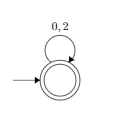
\includegraphics[width=4cm]{FA20/images/fractals/cantor-automata.png}
    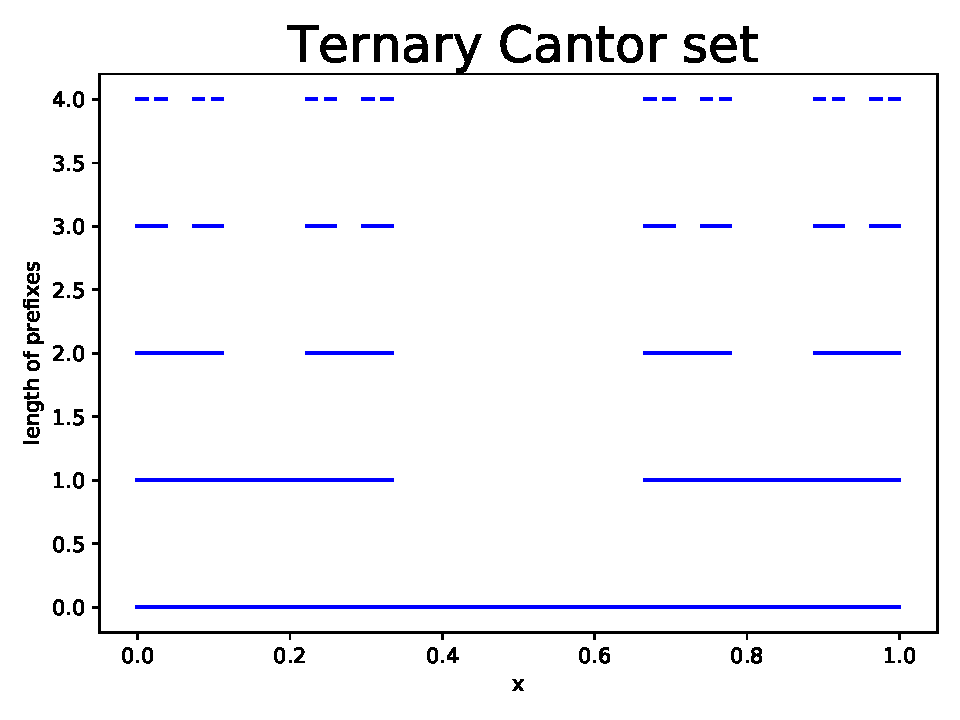
\includegraphics[width=6cm]{FA20/images/fractals/cantor3.pdf}
\end{center}

With a very similar automata (only by changing the accepting words), we can get the Sierpinski Carpet, the Pascal's Triangle, the Menger Sponge, and the Vicsek fractals:

\begin{center}
    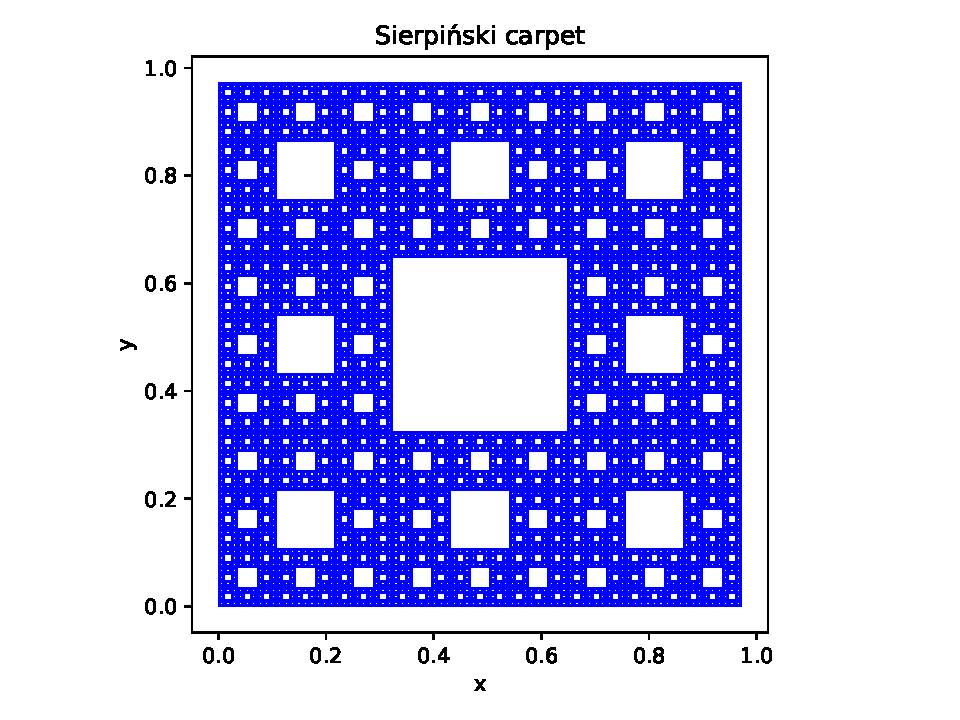
\includegraphics[width=4cm]{FA20/images/fractals/sierpinski-3-l5.pdf}
    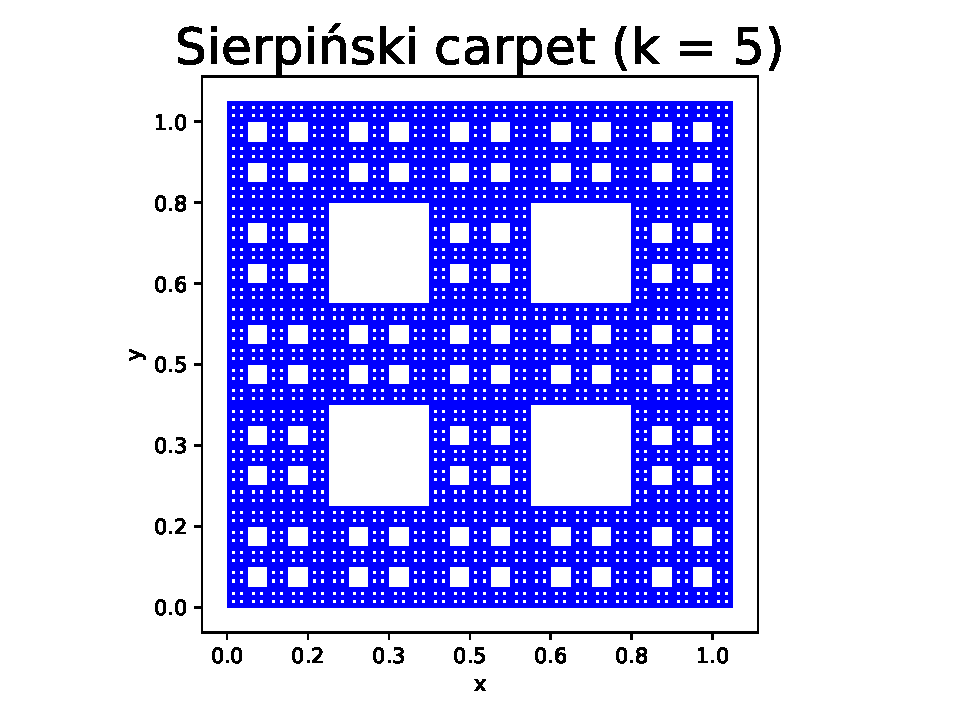
\includegraphics[width=4cm]{FA20/images/fractals/sierpinski-5-l3.pdf}
    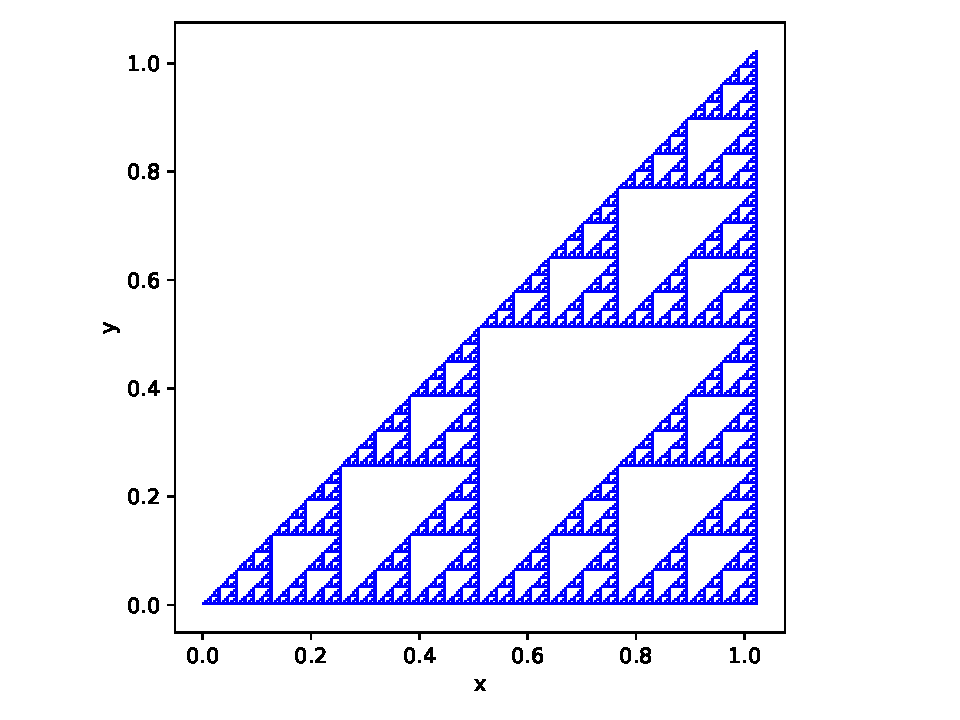
\includegraphics[width=4cm]{FA20/images/fractals/pascal2.pdf}\\
    \includegraphics[width=4cm]{FA20/images/fractals/menger-3-l4.png}
    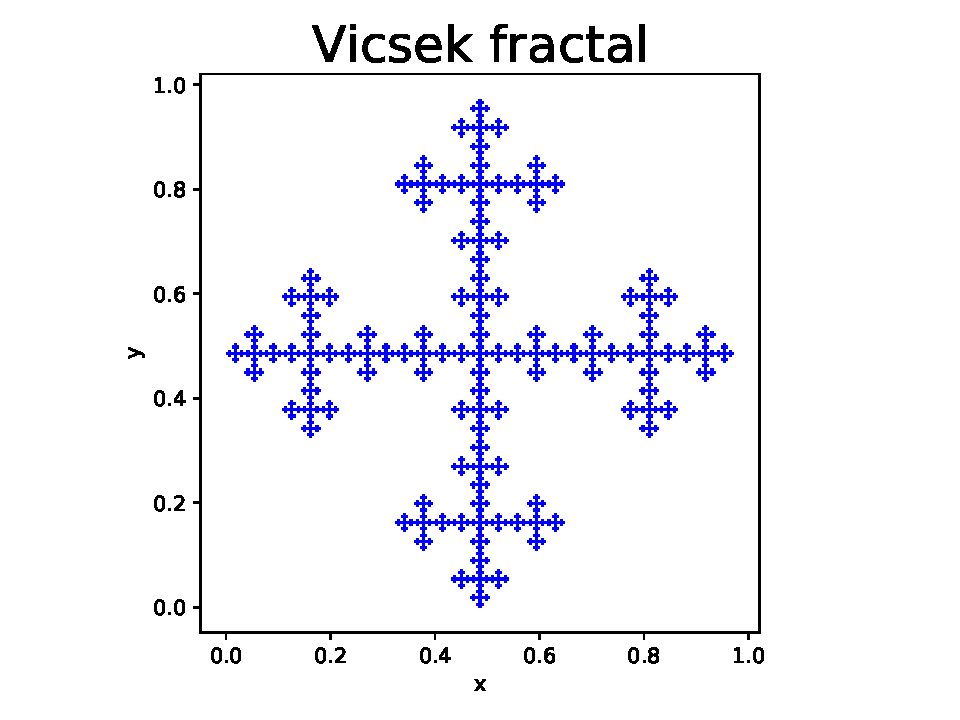
\includegraphics[width=4cm]{FA20/images/fractals/vicsek-l5.pdf}
    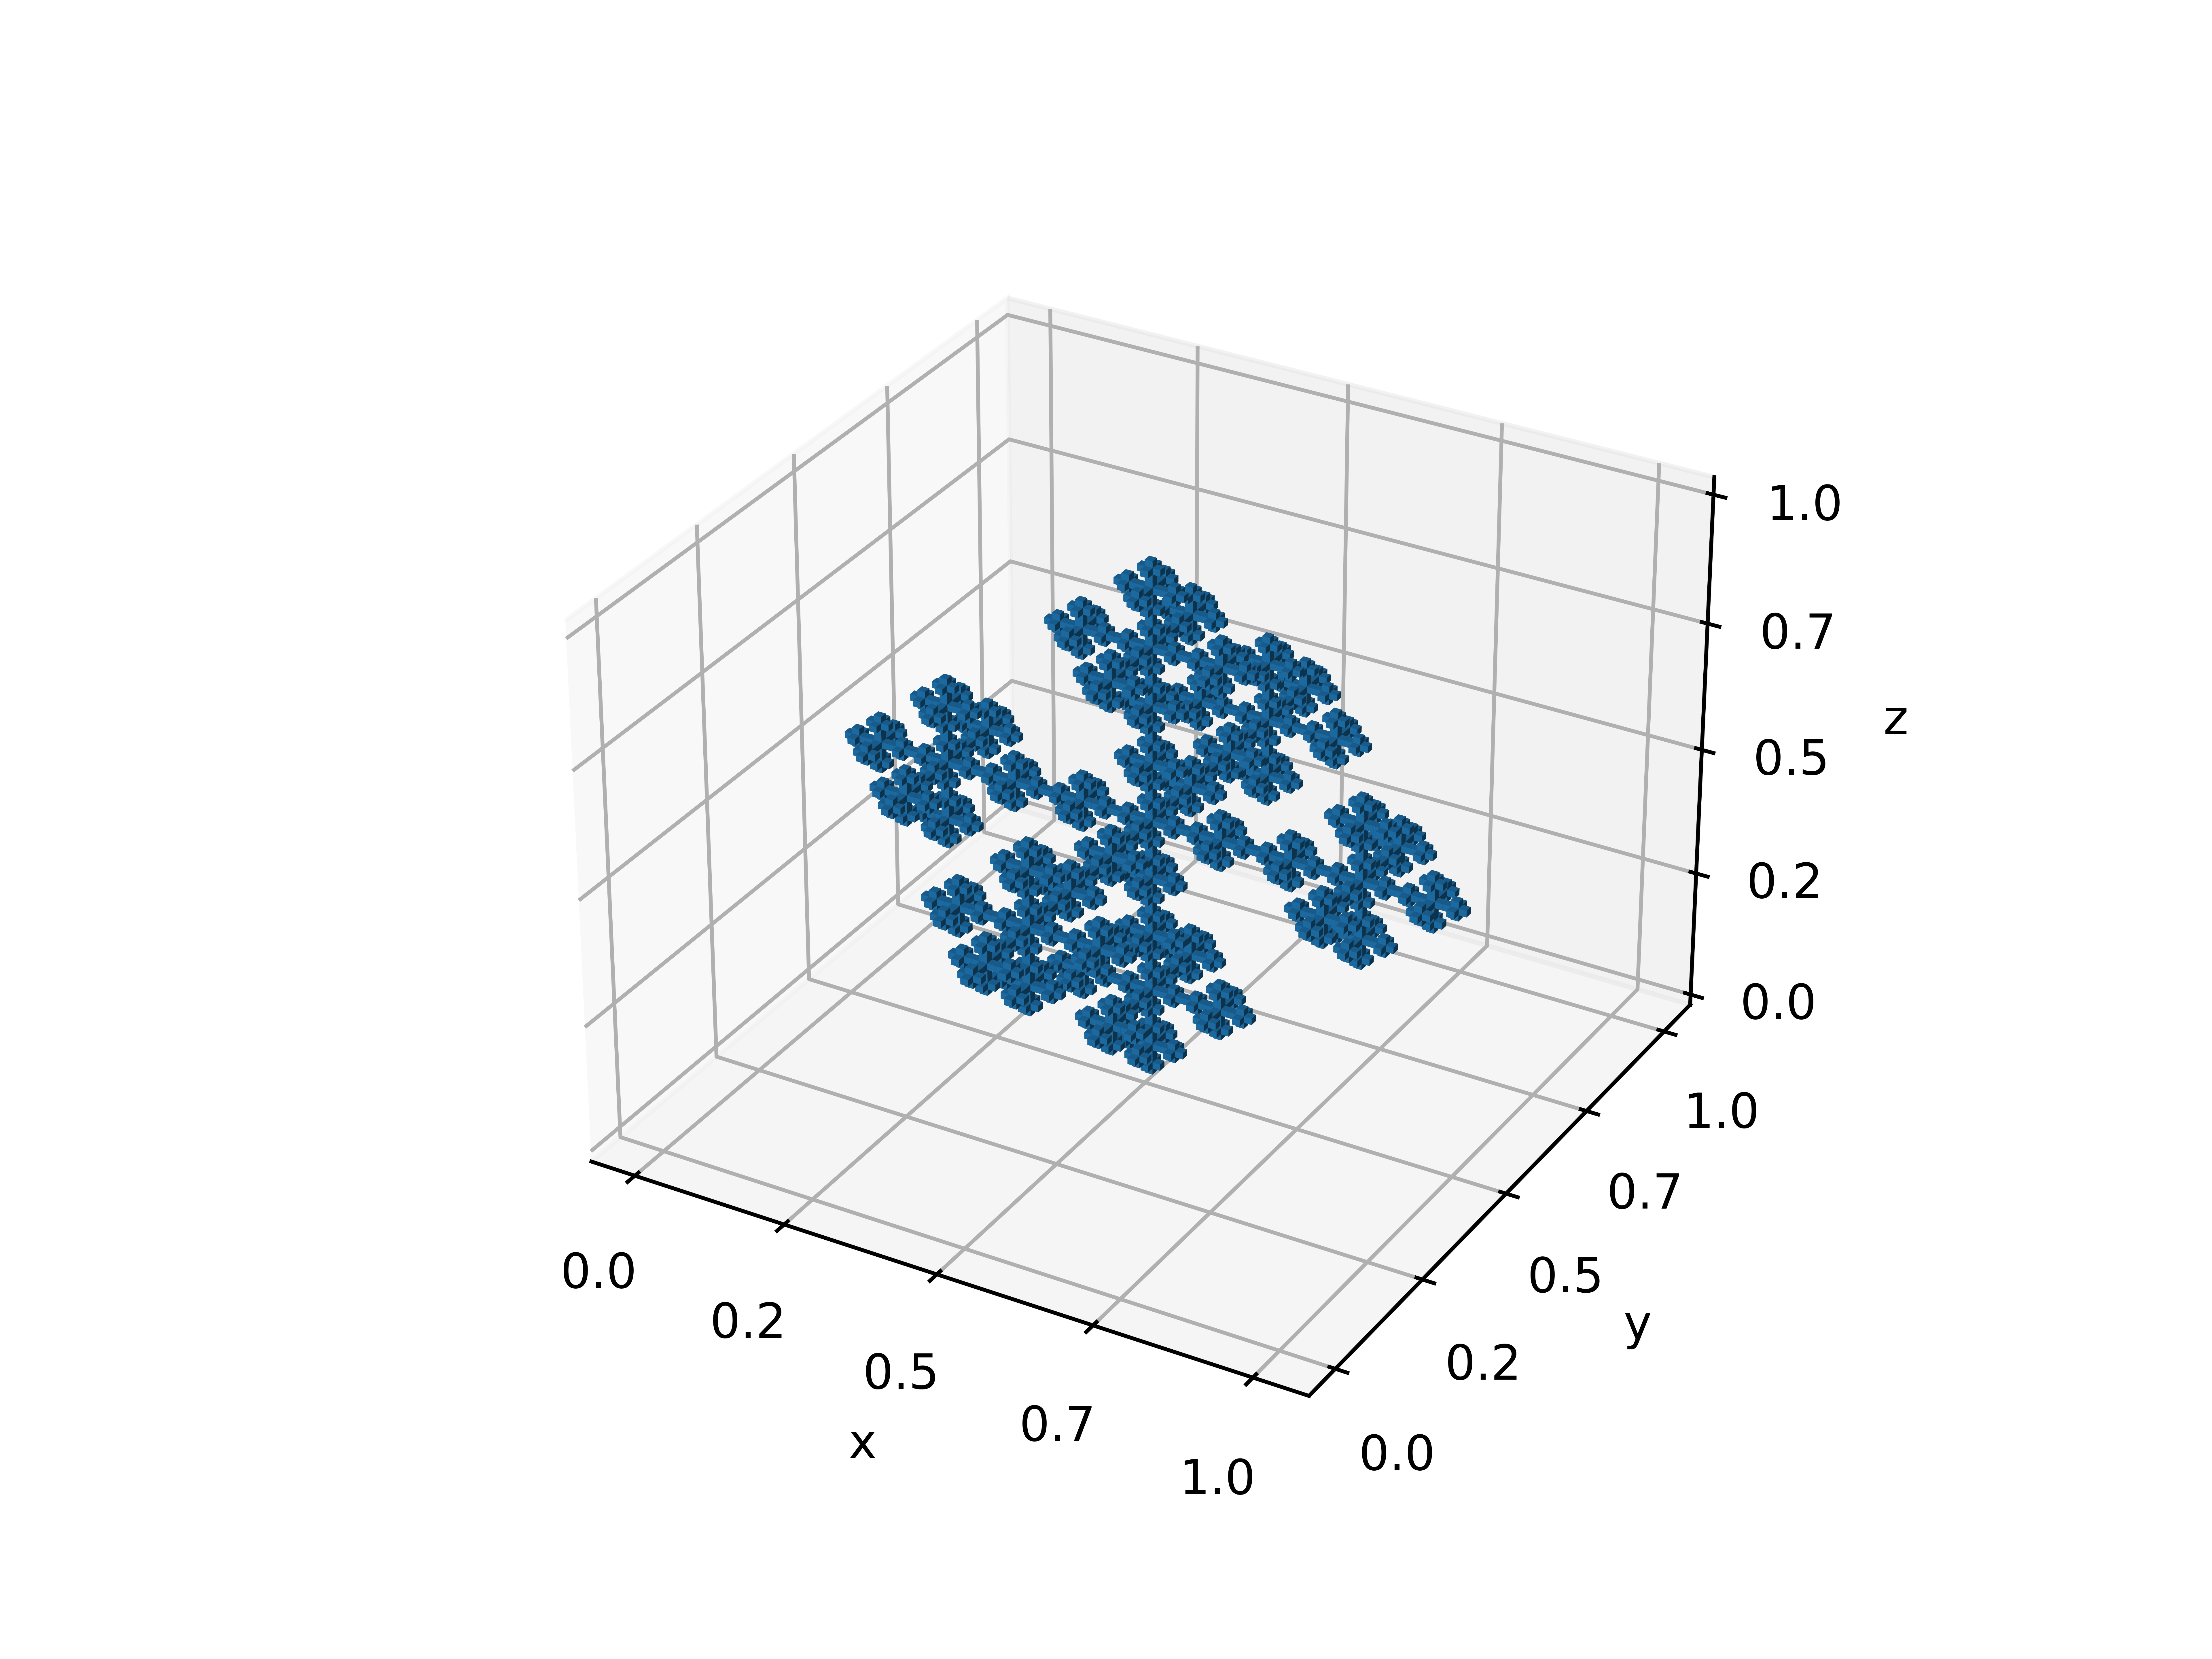
\includegraphics[width=4cm]{FA20/images/fractals/vicsek-3d-l4.png}
\end{center}

If we denote the Cantor set as $C$, we can define a distance function $d:[0,1]\rightarrow [0,1/6]$ by $d(x) = d(x,C) = min_{y \in C}(x,y)$. This function can be represented by the following automata: 

\begin{center}
    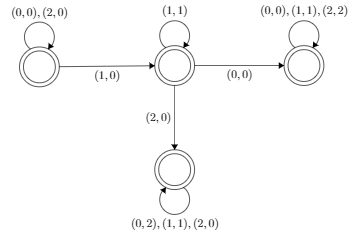
\includegraphics[width=6cm]{FA20/images/fractals/cantord-automata.png}
    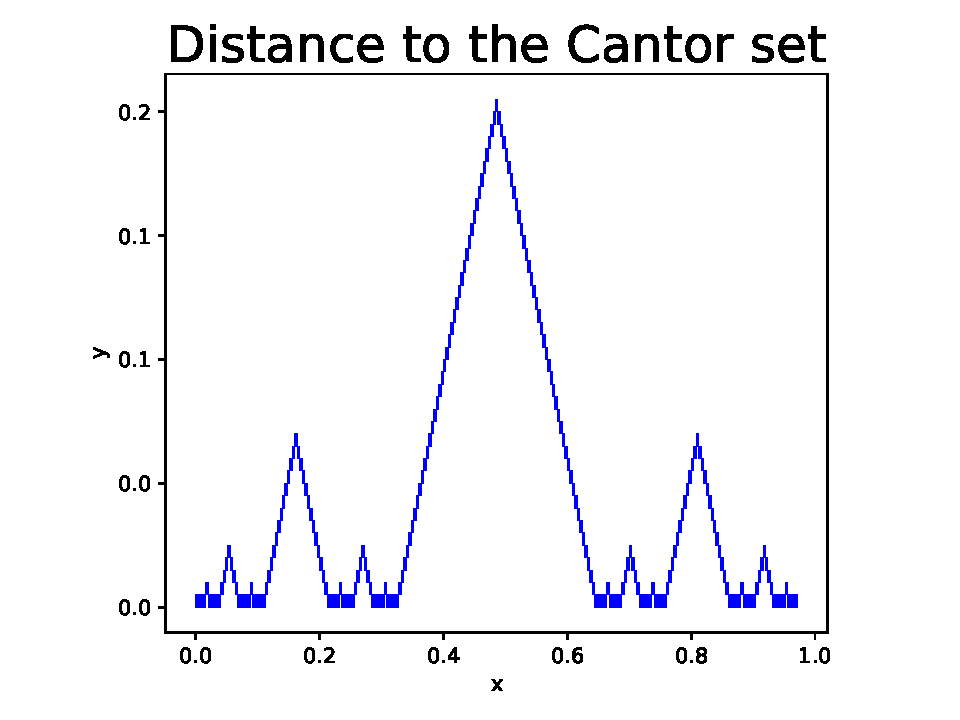
\includegraphics[width=6cm,height=4cm]{FA20/images/fractals/cantord.pdf}
\end{center}

We can also use this function to draw space filling curves like the Hilbert Curve and the Peano Curve. By setting an addition time coordinate, we can think of the Hilbert Curve as a $(2,4)$-regular automata and the Peano Curve a $(3,9)$-regular automata, as follows:

\begin{center}
    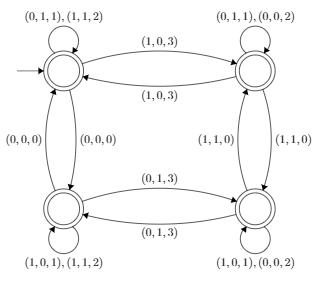
\includegraphics[width=5cm]{FA20/images/fractals/hilbert-automata.png}
    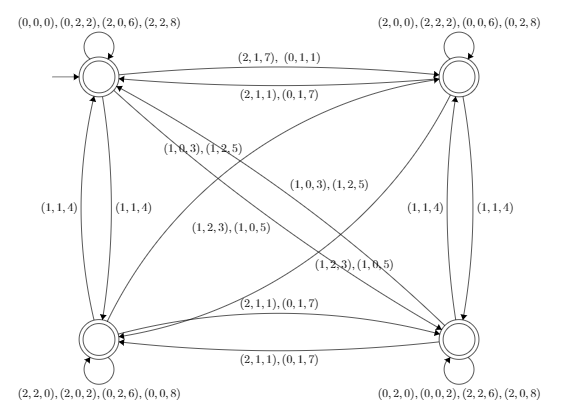
\includegraphics[width=6cm]{FA20/images/fractals/peano-automata.png}
\end{center}

With these automata, we get the following 3 dimensional plots for Hilbert curves (row 1) and Peano Curves (row 2):

\begin{center}
    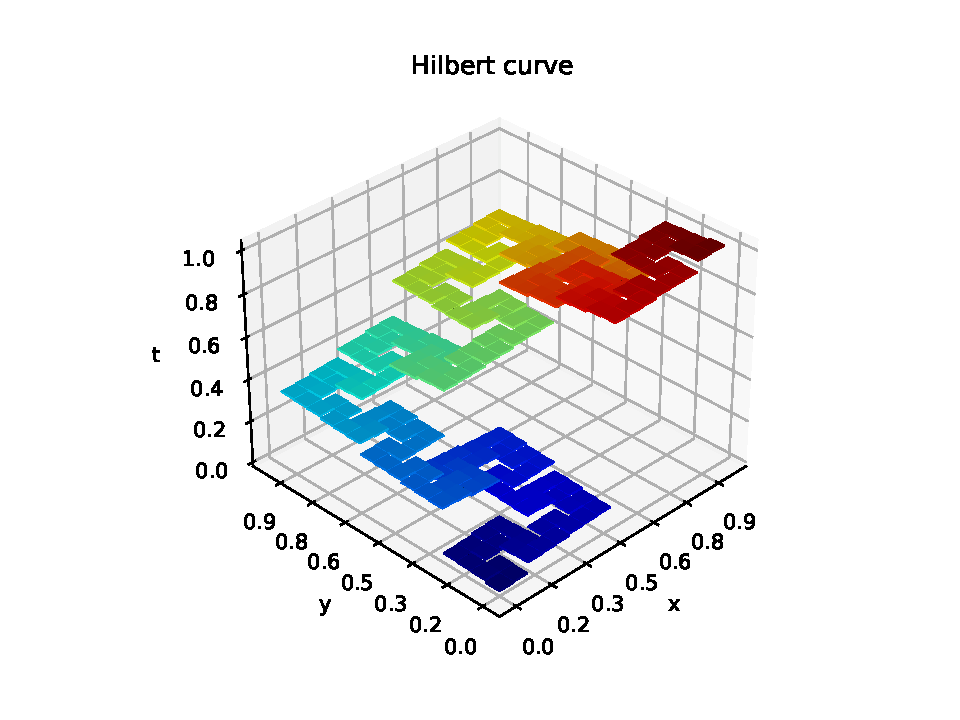
\includegraphics[width=5cm]{FA20/images/fractals/hilbert-1.pdf}
    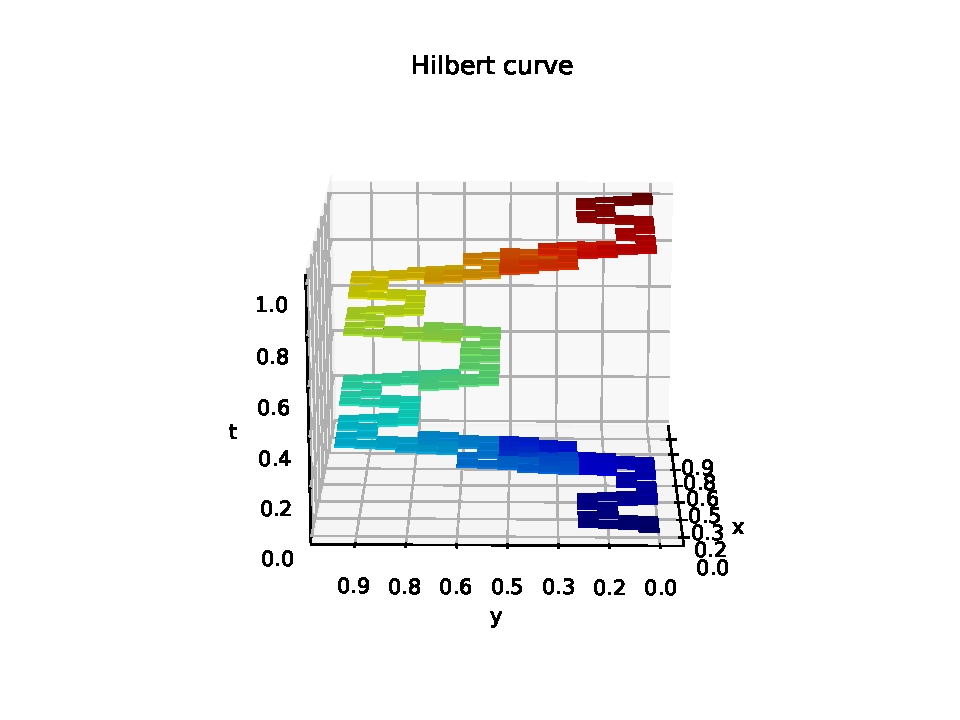
\includegraphics[width=5cm]{FA20/images/fractals/hilbert-2.pdf}
    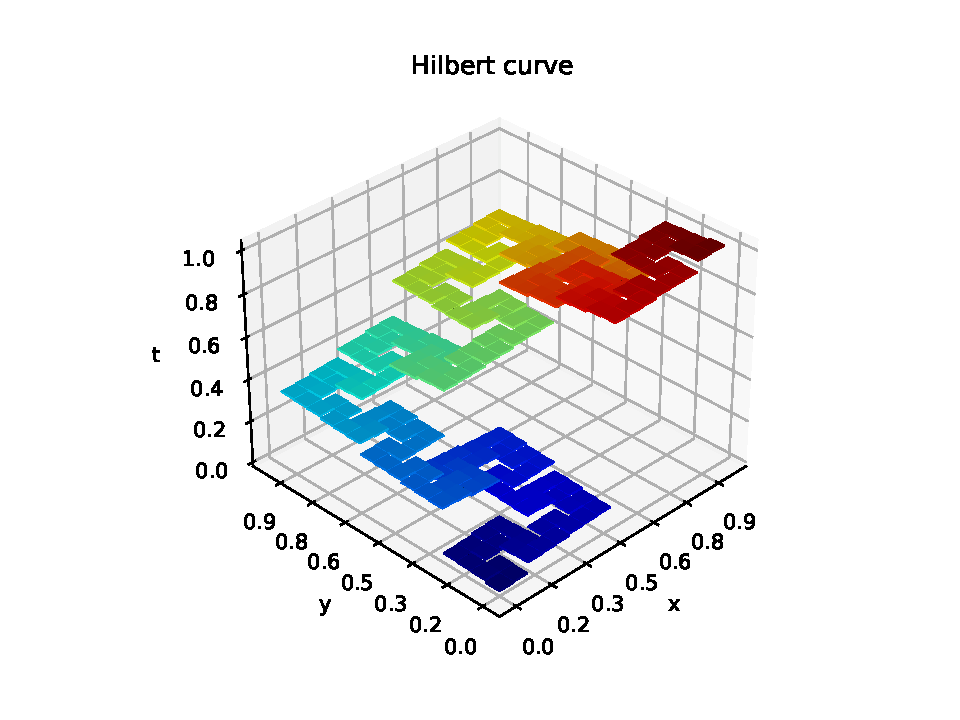
\includegraphics[width=5cm]{FA20/images/fractals/hilbert-1.pdf}\\
    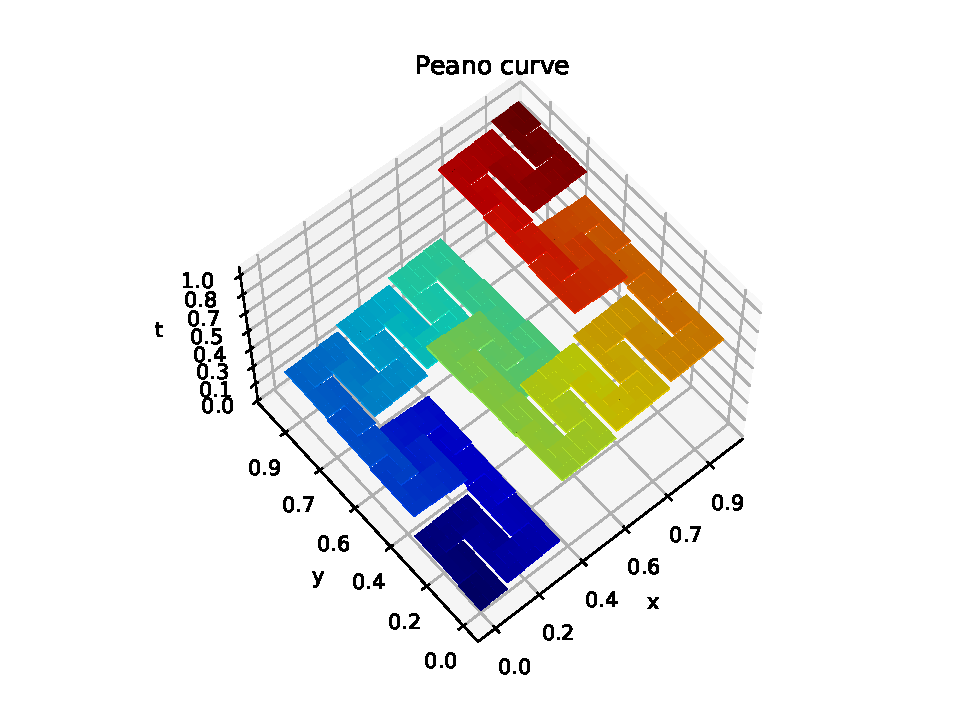
\includegraphics[width=5cm]{FA20/images/fractals/peano-1.pdf}
    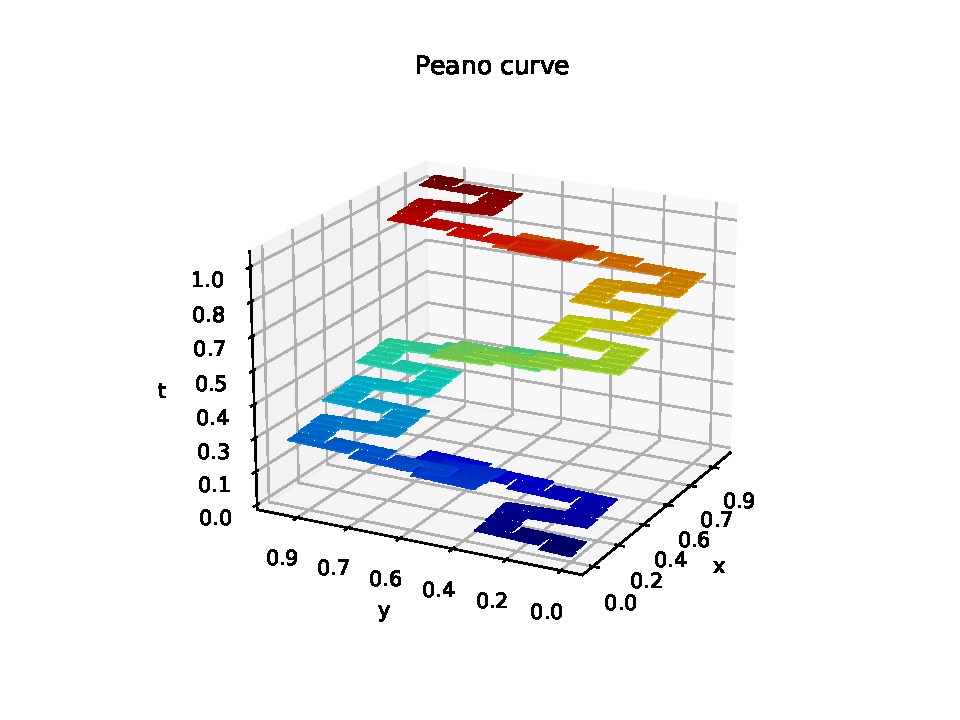
\includegraphics[width=5cm]{FA20/images/fractals/peano-2.pdf}
    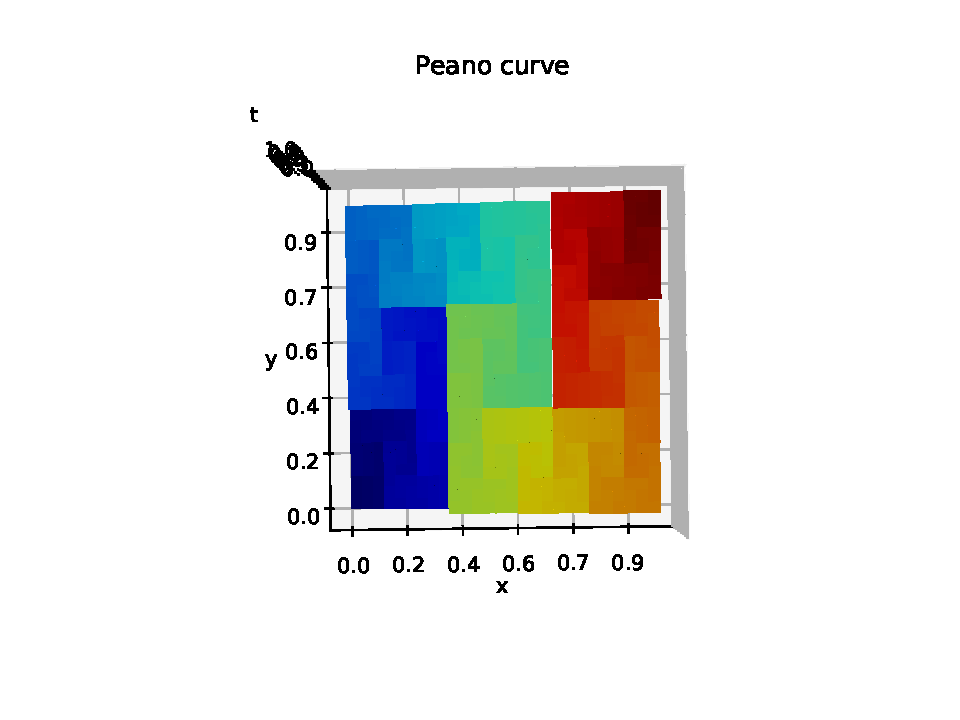
\includegraphics[width=5cm]{FA20/images/fractals/peano-3.pdf}\\
\end{center}

This function should be able to visualize any regular automata. 
We plan to try visualizing more complicated fractals, like Reverend Back's Abbey Floor.

\section{Future Work}

We plan to continue to develop Pecan.
We plan to use Pecan to develop tools that allow working with constraint problems involving non-rational coefficients.
We also plan to continue to develop tools for visualizing fractals, and explore potential applications of these tools.

\section*{Acknowledgements}
Support for this project was provided by the Illinois Geometry Lab and the Department of Mathematics at the University of Illinois at Urbana-Champaign. 
This project was partially supported by NSF grant DMS-1654725. Any opinions, findings, and conclusions or recommendations expressed in this material are those of the author(s) and do not necessarily reflect the views of the National Science Foundation.

\printbibliography

\end{document}
